\documentclass[11pt]{article}
\usepackage{amsmath, amssymb, amsthm}
\usepackage{graphicx}
\usepackage{float}

\begin{document}

\section*{Problem 1 --- Linear Regression / SVD}

\noindent\textbf{(a)} The empirical squared-loss risk is
\begin{align*}
\hat R(w) &= \frac{1}{2n}\sum_{i=1}^d \sum_{j=1}^{n_i} (w_i - y_{ij})^2.
\end{align*}
Differentiating coordinate-wise and setting to zero gives
\begin{align*}
w_i = \frac{1}{n_i}\sum_{j=1}^{n_i} y_{ij}.
\end{align*}

\noindent\textbf{(b)} With $X = \sum_{t=1}^r s_t u_t v_t^\top$ and $y \in \text{span}\{u_1,\dots,u_r\}$, let
\begin{align*}
w = \sum_{t=1}^r \frac{\beta_t}{s_t} v_t, \qquad \text{where } y = \sum_{t=1}^r \beta_t u_t.
\end{align*}
Then
\begin{align*}
Xw = y,
\end{align*}
so the empirical risk is zero.
\vspace{1em} 
\newline
\noindent\textbf{(c)} The nonzero eigenvalues of $X^\top X$ are $s_1^2,\dots,s_r^2$.  
If the rows of $X$ span $\mathbb{R}^d$, then $\text{rank}(X)=d$ and $X^\top X$ is invertible.  
Conversely, if $X^\top X$ is invertible, then $\text{rank}(X)=d$, hence the rows span $\mathbb{R}^d$.

\vspace{1em} 

\noindent\textbf{(d)} Example:
\begin{align*}
X &= \begin{pmatrix} 1 & 0 \\ 0 & 1 \\ 0 & 0 \end{pmatrix}, \qquad
X^\top X = I_2 \ \text{(invertible)}, \qquad
XX^\top = \begin{pmatrix} 1 & 0 & 0 \\ 0 & 1 & 0 \\ 0 & 0 & 0 \end{pmatrix} \ \text{(not invertible)}.
\end{align*}

\section*{Problem 2 --- Linear Regression}

\noindent\textbf{(a), (b)} \quad [skiped: code]
\noindent\textbf{(c)} 

\begin{figure}[H]
  \centering
  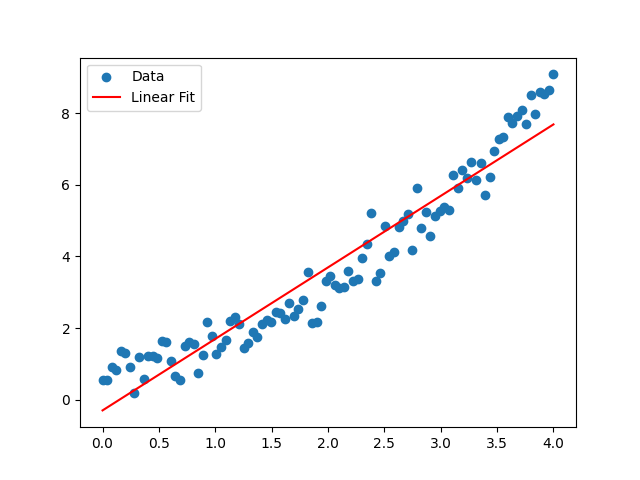
\includegraphics[width=0.7\linewidth]{2-c-output.png}
  \caption{Linear fit and data (Problem 2(c))}
  \label{fig:2c-linear-fit}
\end{figure}

\section*{Problem 3 --- Polynomial Regression}

\noindent\textbf{(a)} For $x=(x_1,x_2,x_3)$,
\begin{align*}
\phi(x) = \big[1,\; x_1,\; x_2,\; x_3,\; x_1^2,\; x_1x_2,\; x_1x_3,\; x_2^2,\; x_2x_3,\; x_3^2\big]^\top.
\end{align*}

\noindent\textbf{(b) to (e)} \quad [skiped: code]

\section*{Problem 4 --- Logistic Regression}

\noindent\textbf{(a)} 
\begin{align*}
\hat R_{\log}(w) &= \frac1n \sum_{i=1}^n \ln\!\big(1+\exp(-y_i w^\top x_i)\big), \\
\nabla_w \hat R_{\log}(w) &= -\frac1n\sum_{i=1}^n y_i x_i\,\sigma(-y_i w^\top x_i), \\
w' &= w + \frac{\eta}{n}\sum_{i=1}^n y_i x_i\,\sigma(-y_i w^\top x_i).
\end{align*}

\noindent\textbf{(b), (c)} \quad [skipped: code]

\section*{Problem 5 --- N-Gram Next Token Prediction (Cross-Entropy)}

\noindent\textbf{(a)} For sample $(x_i,y_i)$ with one-hot target $e_{y_i}$,
\begin{align*}
\nabla_W \ell_i(W) &= x_i\big(p(\cdot|x_i)-e_{y_i}\big)^\top, \\
\nabla_W \hat R_{\mathrm{CE}}(W) &= \frac1n \sum_{i=1}^n x_i\big(p(\cdot|x_i)-e_{y_i}\big)^\top, \\
W' &= W - \frac{\eta}{n} \sum_{i=1}^n x_i\big(p(\cdot|x_i)-e_{y_i}\big)^\top.
\end{align*}

\noindent\textbf{(b) to (e)} \quad [skipped: code]

\section*{Problem 6 --- LLM Use, Collaboration, and Other Sources}

\begin{enumerate}
\item An AI assistant was used in Problems 1(a--d), 4(a), and 5(a). Final answers were edited and wrapped up manually on my ipad. Then, used AI to reformat into Latex.
\item The assignment handout was referenced for problem statements and notation.
\item No additional external sources or collaborators were used.
\end{enumerate}

\end{document}
